\chapter{Teoría del Metamodelado}

El objetivo principal durante la construcción de un metamodelo es aprender un mapeo de la forma $y = f(\mathbf{x})$, donde $f$ es un modelo de caja negra, que puede estudiarse en términos de sus entradas y salidas, pero del que no se tiene un conocimiento explicito de su funcionamiento interno (véase la Fig. \ref{fig:blackboxmodel}). Para modelos de sistemas físicos, este modelo de caja negra oculta las relaciones que transforman el vector de entrada $\mathbf{x}$ en la variable escalar $y$ que es medida, y puede tener una o varias de las siguientes propiedades:
\begin{itemize}
\item El número de experimentos que pueden realizarse es limitado.
\item Cada instancia de un experimento es costosa de ejecutar o puede dañar o destruir el sistema.
\item El resultado de un experimento está sujeto a ruido y/o errores.
\item Dado $\mathbf{x}\in D \subset \mathbf{R}^n$, $n$ puede ser un valor arbitrariamente grande que requiera de un número exponencial de experimentos, si se quiere cubrir de manera uniforme el dominio $D$.
\end{itemize}

\begin{figure}[hbt]
\centering
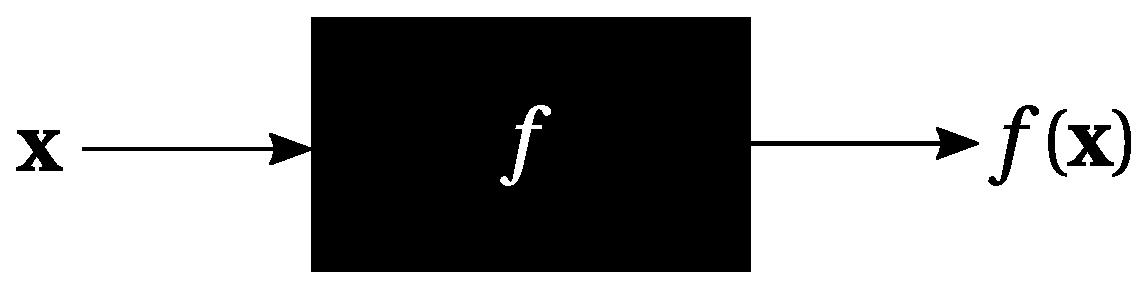
\includegraphics[scale=0.25]{../img/Construccion_de_un_Metamodelo/blackboxmodel.eps}
\caption{Representación de un modelo de caja negra.}
\label{fig:blackboxmodel}
\end{figure}

En este sentido, ``aprender el mapeo'' puede verse como un problema de ajuste de curva (\textit{curve fitting}) para sistemas simples, o de aprendizaje de máquina (\textit{machine learning}) \cite{forrester2008}. En específico, el aprendizaje del mapeo se realiza a partir de \textit{observaciones} o \textit{muestras}, que son el resultado de experimentos. De esta forma, si $E$ es un conjunto de entrenamiento de $k$ muestras, obtenidas al ejecutar $k$ experimentos, entonces este conjunto puede definirse como
\begin{equation*}
E = \lbrace \mathbf{x}^{(i)}\rightarrow y^{(i)}=f(\mathbf{x}^{(i)})|i=1,2,\ldots,k \rbrace
\end{equation*}
De esta forma se cuenta con pares $(\mathbf{x}^{(i)},y^{(i)})$ que pueden utilizarse durante el aprendizaje del mapeo, en lo que consiste un ejercicio de \textit{aprendizaje supervisado} \cite{hastie2008}. El resultado de este aprendizaje es un nuevo modelo: el metamodelo $\hat{f}(\mathbf{x})$. Se han propuesto diferentes estructuras para este modelo, como polinomios, funciones de base radial, modelos Kriging, redes neuronales, máquinas de soporte vectorial y sistemas difusos, entre otros \cite{forrester2008,tenne2010}. El metamodelo obtenido tiene, idealmente, las siguientes características:
\begin{itemize}
\item Varios órdenes de magnitud más rápido de evaluar que el sistema modelado.
\item Minimización del error entre la salida del metamodelo y la salida real del modelo sobre el conjunto de entrenamiento.
\item Generalización en puntos no incluidos en el conjunto de entrenamiento: el metamodelo podría capturar la naturaleza del modelo.
\item En algunos casos su estructura puede revelar relaciones entre las entradas y la salida, a través de parámetros como los coeficientes de un polinomio, o los pesos de las entradas de una red neuronal.
\end{itemize}

Los pasos para la construcción de un metamodelo se muestran en la Fig. \ref{fig:metamodelingsteps}. El primer paso consiste en el análisis de la influencia de las variables de entrada en la salida (en la literatura este proceso se conoce como \textit{feature screening} o \textit{feature extraction}). Debido a que es de interés reducir el número de experimentos que deben realizarse para construir el metamodelo, es necesario verificar que cada una de las $n$ variables tenga efectivamente una influencia en la salida, con el fin de eliminar variables que únicamente pueden incrementar el costo computacional del proceso, sin aportar información adicional para la construcción del metamodelo. Este proceso puede realizarse por medio de la evaluación del coeficiente de correlación R$^2$ de cada una de las variables \cite{giurgea2007}, los p-valores \cite{meng2010} y análisis de varianza (ANOVA) \cite{gillon2010}, entre otros, mientras que para problemas de alta dimensionalidad ($n \gg 10$) se puede realizar un análisis secuencial de parámetros \cite{silva2015}.

\begin{figure}[t]
\centering
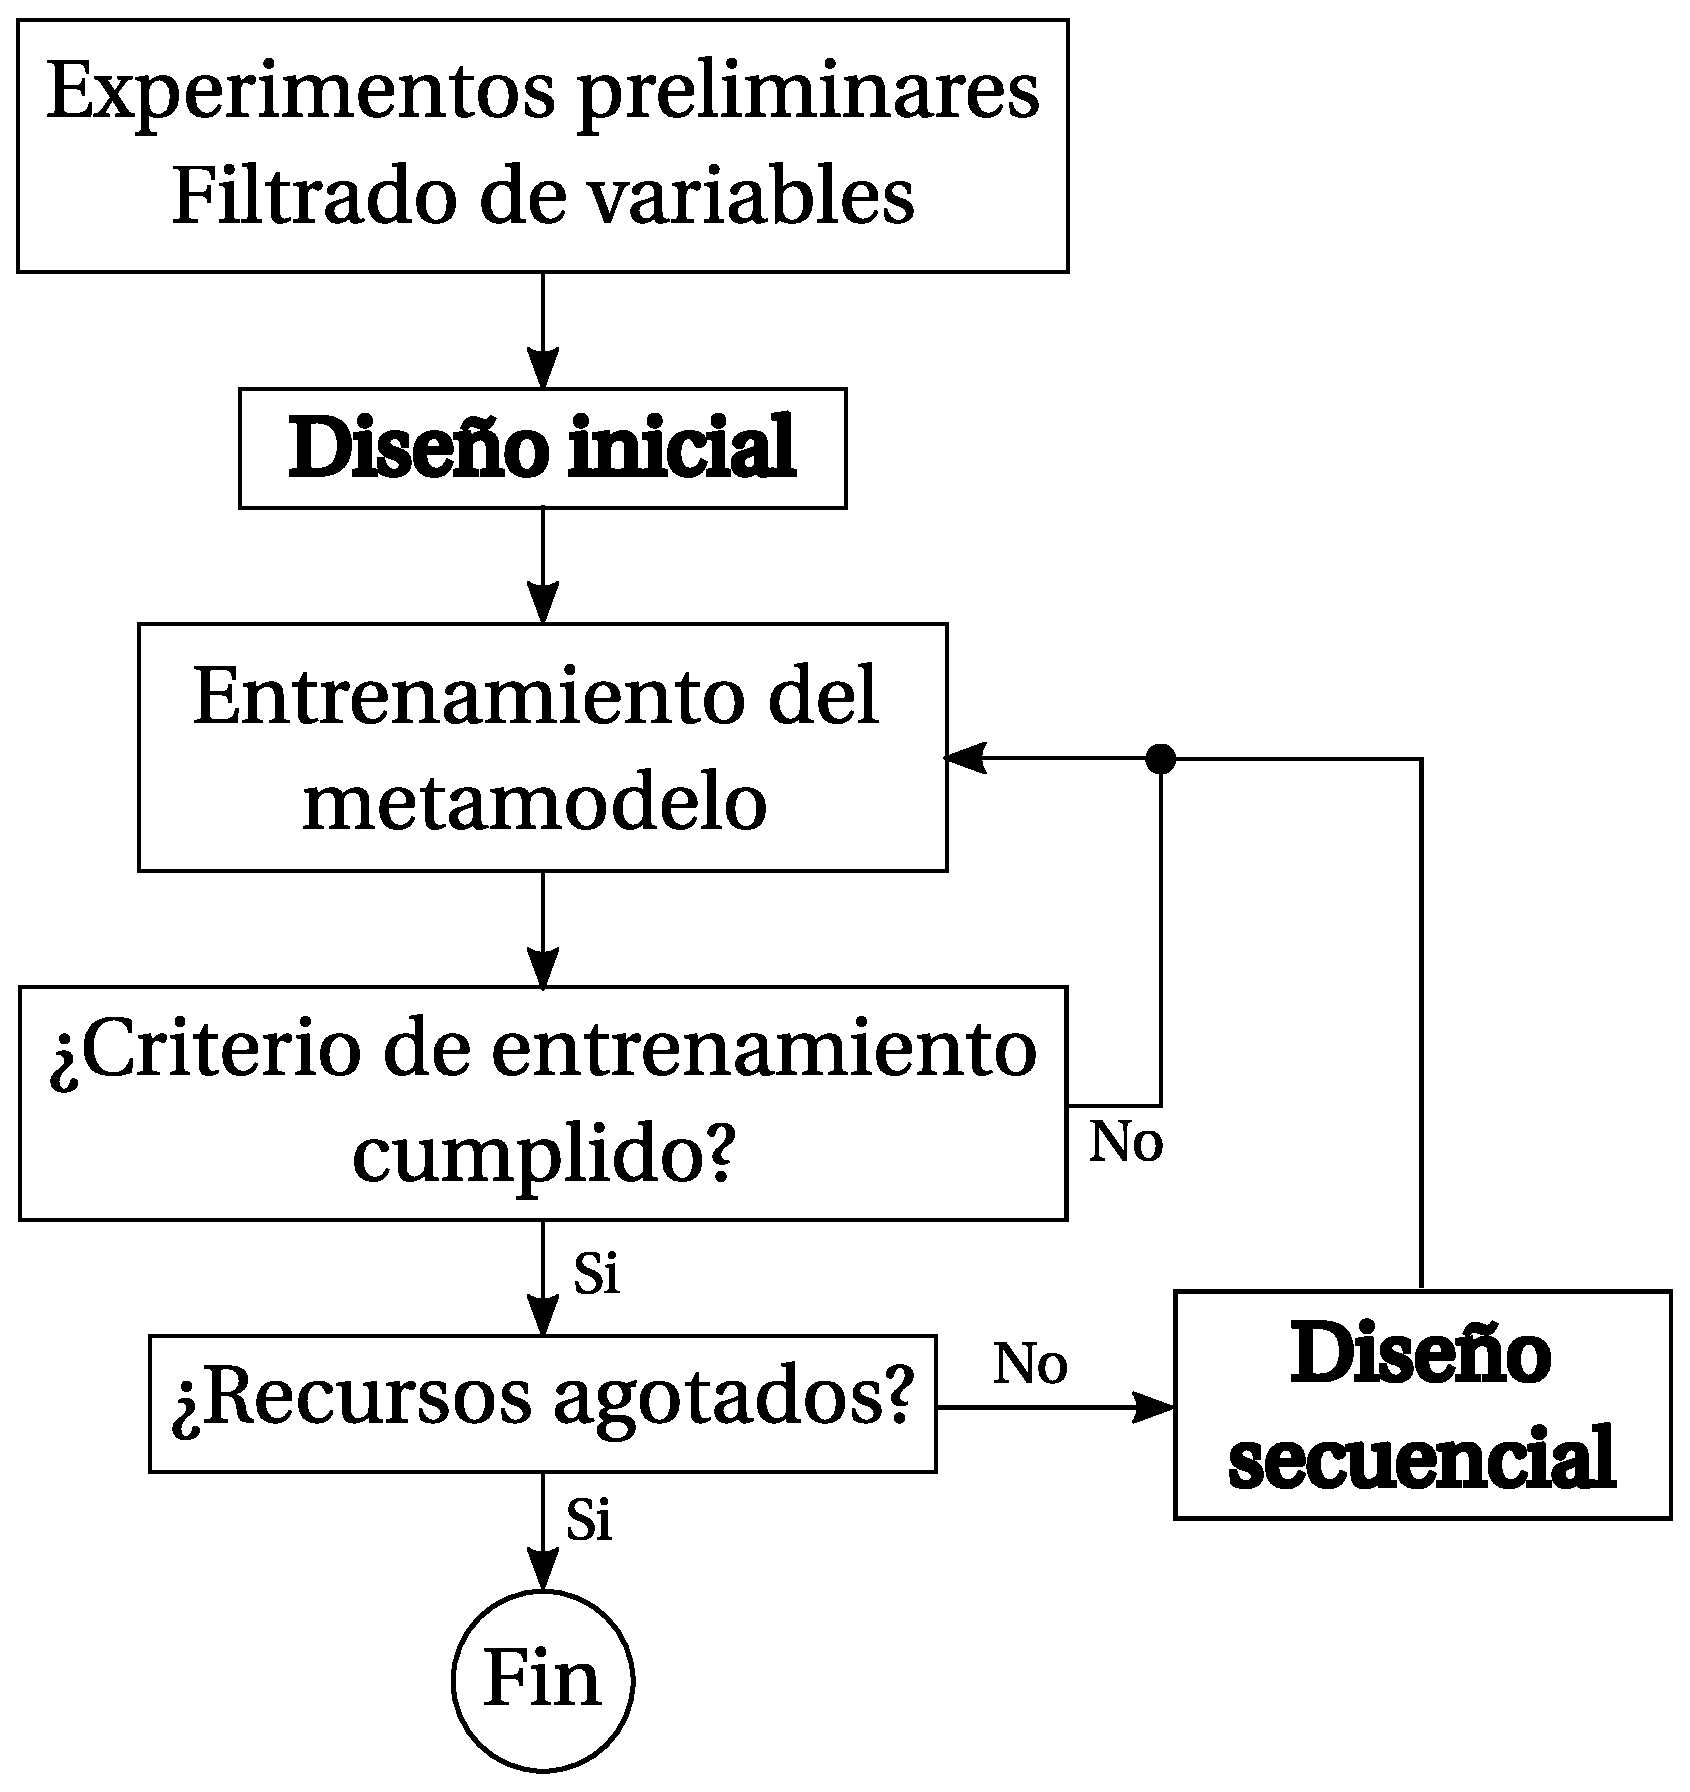
\includegraphics[scale=0.28]{../img/Construccion_de_un_Metamodelo/metamodelingsteps.eps}
\caption{Diagrama de flujo para la construcción de un metamodelo. Los pasos en negrita indican pasos en los que se ejecutan experimentos en el sistema.}
\label{fig:metamodelingsteps}
\end{figure}

Una vez se han seleccionado las variables más importantes, se pasa al \textbf{diseño de experimentos}, donde se crea un plan que define cuáles puntos en el espacio de diseño se van a explorar \cite{montgomery2013}, y que son evaluados a partir de la ejecución de experimentos por medio del sistema a modelar. Cómo se mencionó en las conclusiones del capítulo anterior, en el contexto de la maldición de la dimensionalidad, es posible muestrear el espacio de diseño de forma uniforme, obteniéndose en total $k^n$ muestras, donde $k$ es el número de niveles en los que cada variable es muestreada (véase la Fig. \ref{fig:dimensionality}). Este método de diseño de experimentos se conoce como diseño \textbf{factorial completo} (o \textit{full factorial design} en la literatura). Aunque el diseño factorial completo es intuitivo y fácil de implementar, produce un gran número de experimentos que pueden ser no muy eficientes a la hora de producir muestras diferentes en el espacio de diseño. Por ejemplo, en la figura \ref{fig:dimensionality2} se observa que las muestras pueden agruparse por columnas de valores de $x_1$ constante, de forma que por cada columna, hay cuatro muestras donde el valor de $x_1$ se mantiene constante.

Como alternativa al diseño factorial completo se pueden utilizar diseños más elaborados, como el diseño de \textbf{hipercubo latino}, el cual se basa en el concepto del cuadrado latino\footnote{Un cuadrado latino tiene una única ocurrencia de un símbolo a lo largo de una fila y una columna. El siguiente cuadrado, por ejemplo, es un cuadrado latino:\\

\centering
\begin{tabular}{|c|c|c|}
\hline
x & y & z\\ \hline
z & x & y\\ \hline
y & z & x\\ \hline
\end{tabular}\\
}. Este tipo de diseño se muestra en la Fig. \ref{fig:dimensionality3}, y es un tipo de diseño que puede generalizarse a dimensiones más altas. Es importante tener en cuenta que no se deben asignar todos los recursos computacionales a la etapa del diseño inicial de experimentos, ya que esta no es la única en la cual es necesario ejecutar experimentos en el sistema, como se verá más adelante durante el diseño secuencial de experimentos.

\begin{figure}[t]
    \centering
    \begin{subfigure}[b]{0.32\textwidth}
    \centering
        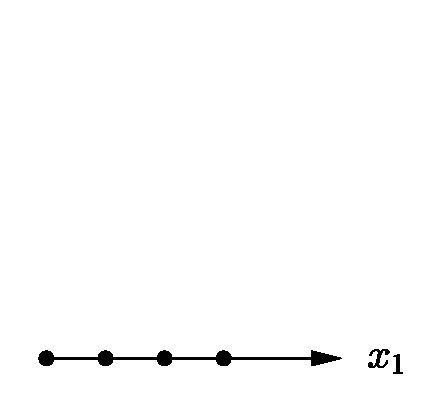
\includegraphics[scale=0.55]{../img/Construccion_de_un_Metamodelo/dimensionality1.eps}
        \caption{$n=1$, $k=4$}
        \label{fig:dimensionality1}
    \end{subfigure}
    ~ %add desired spacing between images, e. g. ~, \quad, \qquad, \hfill etc. 
      %(or a blank line to force the subfigure onto a new line)
    \begin{subfigure}[b]{0.32\textwidth}
    \centering
        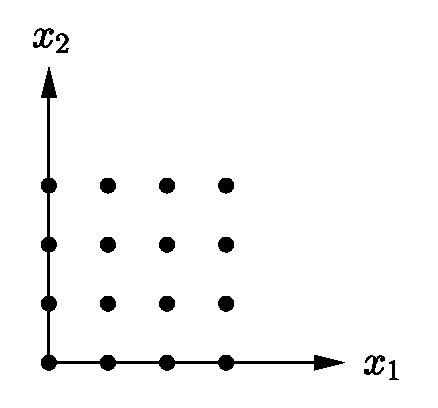
\includegraphics[scale=0.55]{../img/Construccion_de_un_Metamodelo/dimensionality2.eps}
        \caption{$n=2$, $k=4$}
        \label{fig:dimensionality2}
    \end{subfigure}
    \begin{subfigure}[b]{0.32\textwidth}
    \centering
        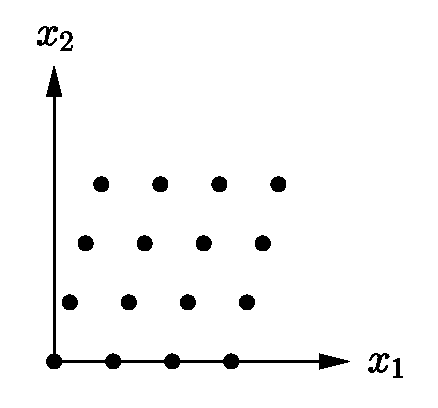
\includegraphics[scale=0.55]{../img/Construccion_de_un_Metamodelo/dimensionality3.eps}
        \caption{Hipercubo latino}
        \label{fig:dimensionality3}
    \end{subfigure}
    \caption{Diseño factorial completo para $n=1$ y $n=2$ y diseño de hipercubo latino.}\label{fig:dimensionality}
\end{figure}

Una vez se ha seleccionado un diseño inicial que plantea un conjunto de muestras a obtener en el espacio de diseño, cada muestra es evaluada en el sistema a modelar, obteniéndose diferentes pares $(\mathbf{x}^{(i)},y^{(i)})$ que forman el primer conjunto de entrenamiento para el metamodelo. La construcción del metamodelo es un proceso iterativo de entrenamiento que depende de su estructura, pero que en general se constituye por dos etapas: una de entrenamiento y otra de evaluación del error (que determina parte del criterio de entrenamiento). En este punto nacen tres preguntas:
\begin{itemize}
\item ¿Qué estructura utilizar para el metamodelo?
\item ¿Cómo entrenarlo?
\item ¿Qué métrica de error utilizar?
\end{itemize}

Las dos primeras preguntas se relacionan con los teoremas planteados por Wolpert y Macready en \cite{NFLT}: no existe una estructura para el metamodelo, ni un método de entrenamiento, que pueda ser seleccionado \textit{a priori}, lo cual explica el por qué el tipo de estructuras encontradas en la literatura es tan variado: funciones de base radial para el modelado de tuberías de gas y máquinas de soporte vectorial para el modelado de antenas de radiofrecuencia \cite{koziel2013}, superficies polinomiales \cite{park2006}, redes neuronales \cite{mohammadi2015} y modelos Kriging \cite{song2011} para motores de reluctancia, y procesos gaussianos para el modelado de sistemas aerodinámicos \cite{zhou2007}, entrenados con técnicas como \textit{backpropagation} en el caso de las redes neuronales, y otros algoritmos como los algoritmos genéticos, optimización por enjambre de partículas y programación cuadrática, entre otros. Aunque pueden presentarse ciertas tendencias en cuanto a la estructura del metamodelo y el método de entrenamiento, como se muestra en el estudio de revisión realizado en \cite{duan2013} en el contexto del diseño de máquinas eléctricas (donde sobresalen el uso de las superficies polinomiales y el algoritmo de evolución diferencial), todos estos resultados invitan a la aplicación de diferentes métodos en una primera aproximación a la construcción del metamodelo.

La siguiente pregunta generalmente es evitada en muchos casos, donde la métrica de error por defecto es el error cuadrático medio (MSE) o su raíz (RMSE). Sin embargo, existen muchas otras métricas de error, tanto absolutas como relativas, que pueden ser de utilidad para la evaluación del metamodelo y que pueden producir resultados muy diferentes, como el error euclidiano promedio, el error geométrico promedio y el error cuadrático relativo, entre otros \cite{gorissen2010}. Por lo tanto, es necesario hacer un estudio del problema a la hora de seleccionar una métrica de error adecuada. Con una métrica de error seleccionada y entendida en el contexto del problema, puede generarse un criterio de entrenamiento para el modelo, al que pueden añadirse criterios adicionales como el número de iteraciones y el tiempo de entrenamiento.

Cuando el ciclo de entrenamiento se ha cumplido, se verifica si los recursos (es decir, el número de experimentos que pueden realizarse en total) se han agotado. Si todavía existen recursos disponibles, se pasa a la etapa de \textbf{diseño secuencial}, razón por la cual no deben utilizarse todos los recursos durante el diseño inicial. Durante la etapa de diseño secuencial se analiza el conjunto de entrenamiento con que se cuenta, en búsqueda de dos características en el espacio de diseño: regiones altamente no-lineales y regiones no exploradas. El énfasis en estos dos tipos de regiones permite obtener un metamodelo que captura satisfactoriamente las no-linealidades del sistema, y que generaliza sus propiedades a lo largo del espacio de diseño. Debido a que los recursos son limitados, esto implica un balance entre \textbf{explotación} (énfasis en regiones no-lineales) y \textbf{exploración} (muestreo uniforme del espacio de diseño). En \cite{crombecq2009} se citan algunos métodos de diseño secuencial pero que resultan ser complicados y costosos computacionalmente, al tiempo que se propone el algoritmo LOLA-Voronoi para cumplir con el balance de exploración-explotación.

Posterior al diseño secuencial, se repite la etapa de entrenamiento del metamodelo y las etapas sucesivas, hasta que los recursos se agotan. Esto concluye la construcción del metamodelo.

\bibliographystyle{ieeetr}
\bibliography{../refs}